\section{Participant 4}

%% MK

\subsection{date \& time}
\begin{table}[ht]
  \begin{tabular}{|P{3cm}|P{3cm}|}
	\multicolumn{2}{c}{\textbf{2016-08-04}}    	\\ \hline
    Start Time      			& End Time   					\\ \hline
   \textbf{10:20:13} 	& \textbf{11:20:41}    	\\ \hline
   \multicolumn{2}{c}{Duration}    						\\ \hline
   \multicolumn{2}{c}{\textbf{01:00:28}} 			\\ \hline
  \end{tabular}
  \newline\newline
  \caption{p4: date and time}\label{dandt4}
\end{table}

\subsection{Questions}
\begin{itemize} 
  \item[\Checkmark] Are you a Student?
  \item[\XSolidBrush] Did you work in a team?
  \item[\XSolidBrush] Did you listen to music?
  \item[\Checkmark] Did you feel tired?
  \item[\Checkmark] Did you enjoy the tasks?
  \item[\XSolidBrush] Did you give all you attention to the tasks?
  \item[\Checkmark] Were you distracted during the tasks?
  \item[\Checkmark] Did you feel stressed
  \item[\XSolidBrush] Do you think the tasks were easy?  
\end{itemize}


\FloatBarrier
\newpage

\subsection{Accelerometer}

\begin{figure}[ht]
	\centering
	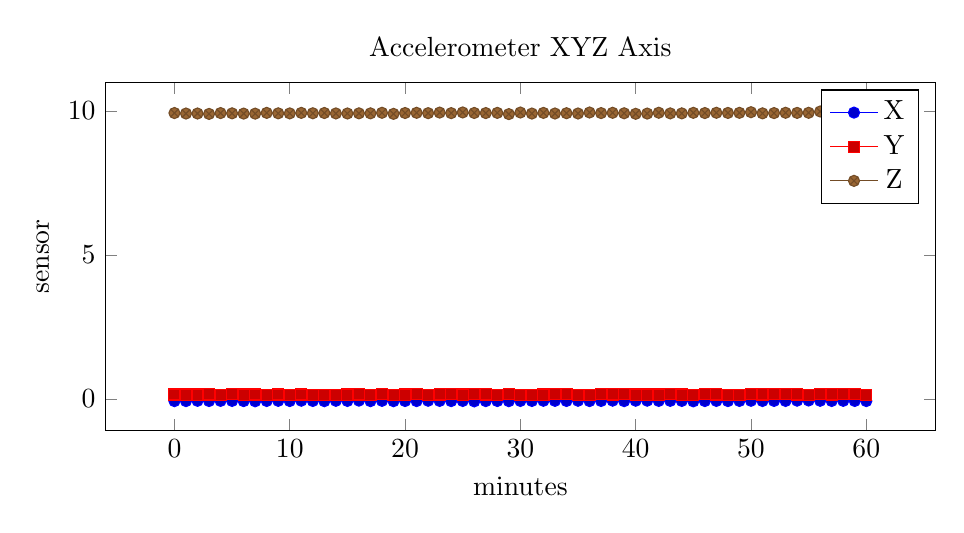
\begin{tikzpicture}
\begin{axis}[
	height=6cm,
	width=\textwidth,
	xlabel=minutes,
	ylabel=sensor,
	title=Accelerometer XYZ Axis,
	unbounded coords=discard],
	
%X
\addplot coordinates {
(0 , -0.0747131762353)
(1 , -0.073247608625)
(2 , -0.063521163625)
(3 , -0.070778586)
(4 , -0.06584054825)
(5 , -0.0672371646667)
(6 , -0.0736217)
(7 , -0.0798067233333)
(8 , -0.0686337833333)
(9 , -0.06434417)
(10 , -0.07122749975)
(11 , -0.0600545593333)
(12 , -0.069282211)
(13 , -0.07631518)
(14 , -0.06299743325)
(15 , -0.0679354745)
(16 , -0.0568622886667)
(17 , -0.07481880275)
(18 , -0.064643445)
(19 , -0.0770134866667)
(20 , -0.0708284676667)
(21 , -0.0723048914)
(22 , -0.061451177)
(23 , -0.0666386146667)
(24 , -0.0737214611667)
(25 , -0.06823475)
(26 , -0.0831985105)
(27 , -0.073621705)
(28 , -0.0700303985)
(29 , -0.07571663)
(30 , -0.06808510825)
(31 , -0.0690328133333)
(32 , -0.06269815775)
(33 , -0.064942722)
(34 , -0.06853402325)
(35 , -0.061052144)
(36 , -0.0724246025)
(37 , -0.0694318475)
(38 , -0.05865794)
(39 , -0.074699092)
(40 , -0.060752869)
(41 , -0.0587576993333)
(42 , -0.066638614)
(43 , -0.065241995)
(44 , -0.0673369215)
(45 , -0.082001406)
(46 , -0.071526772)
(47 , -0.06688800775)
(48 , -0.072723875)
(49 , -0.067636197)
(50 , -0.06314707)
(51 , -0.06958148675)
(52 , -0.0672371633333)
(53 , -0.068035233)
(54 , -0.0580593925)
(55 , -0.0528434535714)
(56 , -0.06254852)
(57 , -0.0688017963684)
(58 , -0.06464344625)
(59 , -0.068234749)
(60 , -0.0725243588333)
};

%Y
\addplot coordinates {
(0 , 0.156256870588)
(1 , 0.15315409)
(2 , 0.15367782375)
(3 , 0.15786767)
(4 , 0.14454993)
(5 , 0.16360378)
(6 , 0.15382746)
(7 , 0.155822623333)
(8 , 0.145846786667)
(9 , 0.155323835)
(10 , 0.15083471)
(11 , 0.155822626667)
(12 , 0.1484405075)
(13 , 0.142455)
(14 , 0.144250655)
(15 , 0.15412673)
(16 , 0.157219246667)
(17 , 0.1415571775)
(18 , 0.160411515)
(19 , 0.147442923333)
(20 , 0.154226496667)
(21 , 0.159214414)
(22 , 0.148240986667)
(23 , 0.157219246667)
(24 , 0.161508855)
(25 , 0.154126735)
(26 , 0.165499195)
(27 , 0.15682021)
(28 , 0.15203181)
(29 , 0.187047005)
(30 , 0.143352825)
(31 , 0.15003664)
(32 , 0.1550245625)
(33 , 0.16011224)
(34 , 0.1593640525)
(35 , 0.15023616)
(36 , 0.14514848)
(37 , 0.16071079)
(38 , 0.15741876)
(39 , 0.162207164)
(40 , 0.15502456)
(41 , 0.15522408)
(42 , 0.153627943333)
(43 , 0.17238252)
(44 , 0.153528185)
(45 , 0.14584679)
(46 , 0.16190789)
(47 , 0.15816695)
(48 , 0.15263036)
(49 , 0.14754268)
(50 , 0.16011224)
(51 , 0.157269125)
(52 , 0.159812963333)
(53 , 0.165997983333)
(54 , 0.15831659)
(55 , 0.147499927143)
(56 , 0.172981075)
(57 , 0.157733788421)
(58 , 0.1634042675)
(59 , 0.1726818)
(60 , 0.140360076667)
};

%Z
\addplot coordinates {
(0 , 9.92474058824)
(1 , 9.9079546875)
(2 , 9.9084784375)
(3 , 9.89433775)
(4 , 9.923517)
(5 , 9.914589)
(6 , 9.905411)
(7 , 9.90421416667)
(8 , 9.93035066667)
(9 , 9.914988)
(10 , 9.91244375)
(11 , 9.930351)
(12 , 9.9172325)
(13 , 9.925762)
(14 , 9.9112465)
(15 , 9.9093015)
(16 , 9.914589)
(17 , 9.91423975)
(18 , 9.9332435)
(19 , 9.89643233333)
(20 , 9.92596133333)
(21 , 9.9329444)
(22 , 9.92097333333)
(23 , 9.940925)
(24 , 9.92167158333)
(25 , 9.9455135)
(26 , 9.9275575)
(27 , 9.92396633333)
(28 , 9.93055)
(29 , 9.8877535)
(30 , 9.94282025)
(31 , 9.907406)
(32 , 9.92965225)
(33 , 9.908703)
(34 , 9.919028)
(35 , 9.90940133333)
(36 , 9.9437185)
(37 , 9.923218)
(38 , 9.932944)
(39 , 9.9166634)
(40 , 9.8985275)
(41 , 9.90640833333)
(42 , 9.935538)
(43 , 9.9128925)
(44 , 9.91379075)
(45 , 9.931947)
(46 , 9.9242655)
(47 , 9.9341415)
(48 , 9.9284555)
(49 , 9.932645)
(50 , 9.954492)
(51 , 9.91409)
(52 , 9.92296833333)
(53 , 9.93414133333)
(54 , 9.930101)
(55 , 9.93345728571)
(56 , 9.9787335)
(57 , 9.92550976316)
(58 , 9.91049875)
(59 , 9.9203745)
(60 , 9.92167166667)
};

\addlegendentry{X}
\addlegendentry{Y}
\addlegendentry{Z}
\end{axis}
\end{tikzpicture}
 	\vspace{5 mm}
\end{figure}

\FloatBarrier
\subsection{Light Level}
\begin{figure}[ht]
	\centering
	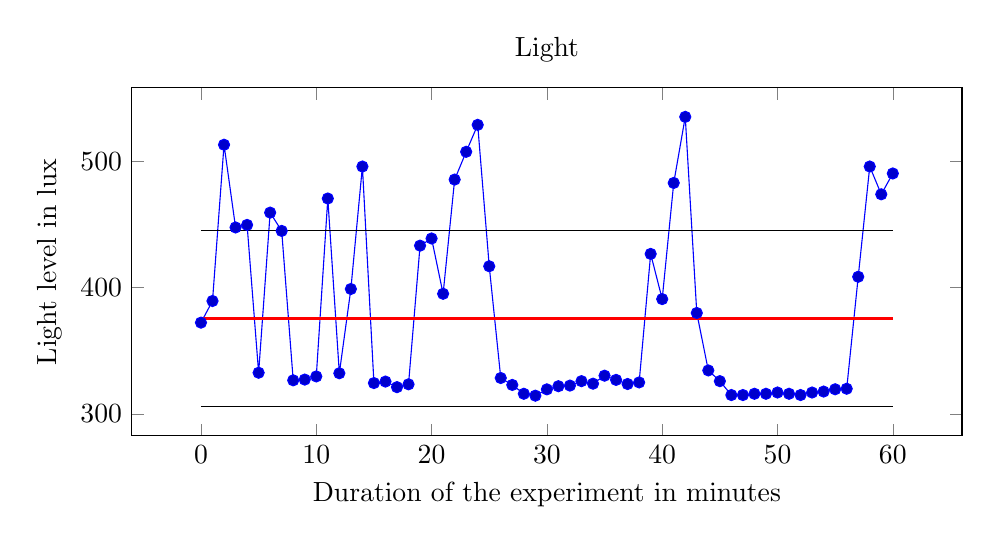
\begin{tikzpicture}
\begin{axis}[
	height=6cm,
	width=\textwidth,
	xlabel=Duration of the experiment in minutes,
	ylabel=Light level in lux,
	title=Light,
	unbounded coords=discard],
	
\addplot coordinates {
(0 , 372.352941176)
(1 , 389.5)
(2 , 513.25)
(3 , 447.75)
(4 , 449.75)
(5 , 332.666666667)
(6 , 459.5)
(7 , 445.0)
(8 , 326.666666667)
(9 , 327.25)
(10 , 329.75)
(11 , 470.666666667)
(12 , 332.25)
(13 , 399.0)
(14 , 496.0)
(15 , 324.5)
(16 , 325.666666667)
(17 , 321.25)
(18 , 323.5)
(19 , 433.333333333)
(20 , 439.0)
(21 , 395.2)
(22 , 485.666666667)
(23 , 507.666666667)
(24 , 529.0)
(25 , 417.0)
(26 , 328.5)
(27 , 323.0)
(28 , 316.0)
(29 , 314.5)
(30 , 319.5)
(31 , 322.0)
(32 , 322.5)
(33 , 326.0)
(34 , 324.0)
(35 , 330.333333333)
(36 , 327.0)
(37 , 323.75)
(38 , 325.0)
(39 , 426.8)
(40 , 391.0)
(41 , 483.0)
(42 , 535.333333333)
(43 , 380.0)
(44 , 334.5)
(45 , 326.0)
(46 , 315.0)
(47 , 315.0)
(48 , 316.0)
(49 , 316.0)
(50 , 317.0)
(51 , 316.0)
(52 , 315.0)
(53 , 317.0)
(54 , 317.75)
(55 , 319.571428571)
(56 , 320.0)
(57 , 408.684210526)
(58 , 496.0)
(59 , 474.0)
(60 , 490.5)
};

\addplot[mark=none, red, very thick] coordinates {(0, 375.580976338) (60, 375.580976338)};

\addplot[mark=none, black] coordinates {(0, 305.697485999) (60, 305.697485999)};
\addplot[mark=none, black] coordinates {(0, 445.464466676) (60, 445.464466676)};


\end{axis}
\end{tikzpicture}
 	\vspace{5 mm}
\end{figure}

\newpage
\FloatBarrier
\newpage
\subsection{Noise Level}
\begin{figure}[ht]
	\centering
	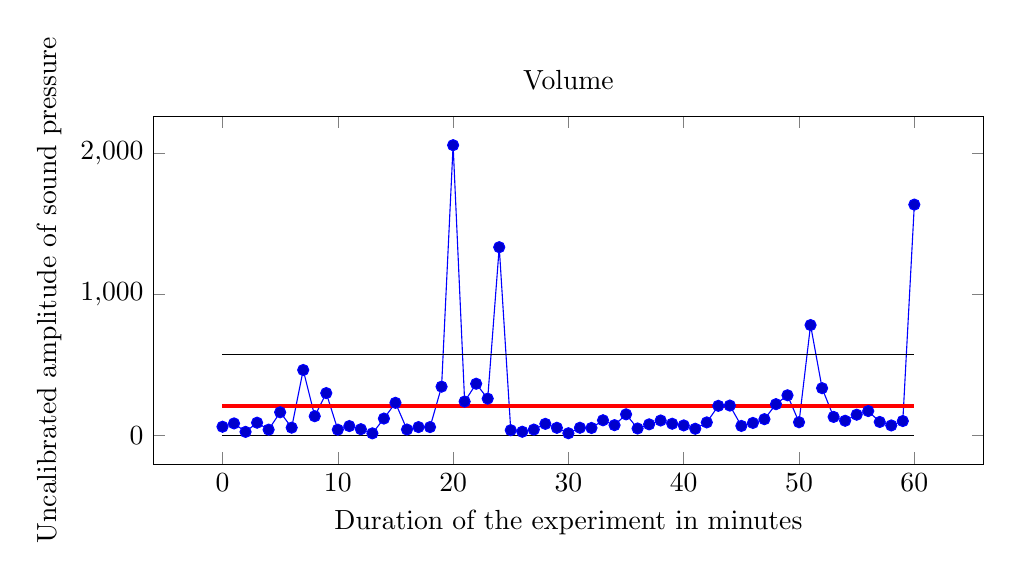
\begin{tikzpicture}
\begin{axis}[
	height=6cm,
	width=\textwidth,
	ylabel=Uncalibrated amplitude of sound pressure,
	xlabel=Duration of the experiment in minutes,
	title=Volume,
	unbounded coords=discard],

\addplot coordinates {
(0 , 59.5882352941)
(1 , 83.125)
(2 , 23.0)
(3 , 88.25)
(4 , 38.75)
(5 , 162.333333333)
(6 , 53.0)
(7 , 462.666666667)
(8 , 134.333333333)
(9 , 298.5)
(10 , 38.5)
(11 , 64.3333333333)
(12 , 42.0)
(13 , 12.5)
(14 , 117.75)
(15 , 229.5)
(16 , 39.6666666667)
(17 , 57.0)
(18 , 57.0)
(19 , 344.333333333)
(20 , 2060.0)
(21 , 238.6)
(22 , 365.0)
(23 , 259.0)
(24 , 1335.16666667)
(25 , 35.0)
(26 , 24.0)
(27 , 39.3333333333)
(28 , 80.0)
(29 , 52.0)
(30 , 13.25)
(31 , 52.3333333333)
(32 , 50.75)
(33 , 105.5)
(34 , 70.75)
(35 , 147.666666667)
(36 , 47.0)
(37 , 76.5)
(38 , 104.0)
(39 , 80.8)
(40 , 69.0)
(41 , 45.1666666667)
(42 , 90.3333333333)
(43 , 208.0)
(44 , 210.0)
(45 , 65.3333333333)
(46 , 86.5)
(47 , 113.25)
(48 , 220.0)
(49 , 283.0)
(50 , 91.5)
(51 , 782.0)
(52 , 333.666666667)
(53 , 129.333333333)
(54 , 102.0)
(55 , 145.0)
(56 , 171.0)
(57 , 93.5789473684)
(58 , 68.75)
(59 , 100.0)
(60 , 1637.83333333)
};

\addplot[mark=none, red, very thick] coordinates {(0, 208.000418295) (60, 208.000418295)};

\addplot[mark=none, black] coordinates {(0, 0) (60, 0)};
\addplot[mark=none, black] coordinates {(0, 571.657643466) (60, 571.657643466)};

\end{axis}
\end{tikzpicture}
 	\vspace{5 mm}
\end{figure}

\FloatBarrier

\subsection{Location}
53.3437734, -6.2510318

Dublin, Ireland 

\FloatBarrier